\ifx\atempxetex\usewhat
\XeTeXinputencoding "utf-8"
\fi
\defaultfont

\chapter{进程管理}

正如第一章所提到的,进程是Unix系统中仅次于文件的基本抽象概念。当目标代码执行的时候,进程不仅仅包括汇编代码,它由数据、资源、状态和一个虚拟的计算机组成。

本章将会讲解一些包括进程从创建到结束的基本概念。自从早期的Unix开始,这些基本的东西就很少发生变化。在进程管理这个主题中,闪烁着Unix设计者们的智慧和远见。在进程的创建上,Unix采取了一种有趣和少见的处理方法:它将进程的创建和加载一个新二进制镜像分离。虽然大多数情况下,这两个任务都是在顺序执行的,但区分后就可以有更多的余地对两种操作进行管理。在大多数操作系统只是简单的提供了一个系统调用创建进程的情况下,这种方式还是保留了下来——Unix提供了两个系统调用fork和exec。但在我们讲解它们之前,还是好好研究一下进程的一些基本概念。

\section{进程ID}

每一个进程都由一个唯一的标识符表示的,即进程ID,简称pid。系统保证在某时刻每个pid都是唯一的。也就是说,在t0时刻有且只有一个进程的pid是770(如果系统中有这样的一个进程的pid是770的话),但是这不代表在t1时刻另一个进程的pid就不能是 770。本质上来讲,大多数代码会假设内核不会重用已经用过的pid值——这个假设,正如你所将看到的,是相当安全的。

空闲进程(idle process)——当没有其他进程在运行时,内核所运行的进程——它的pid是0。在启动后,内核运行的第一个进程称为init进程,它的pid是1。一般来说,Linux中init进程就是init 程序。我们将会使用“init”术语表示内核运行的第一个进程和完成相应目的特定程序。

除非用户显式地指定内核所要运行的程序(通过内核启动的init参数),否则内核就必须寻找一个适合的init程序——这是很少见的内核特定要求中的一个例子。Linux内核会以以下顺序进行尝试:

\begin{enumerate}
\item /sbin/init:init最有可能存在的地方。
\item /etc/init:另一个可能的地方。
\item /bin/init:init一个可能存在的位置。
\item /bin/sh:Bourne shell的所在的位置,当内核没有找到init时,内核就会尝试运行它。
\end{enumerate}

在以上候选位置中,第一被发现的就会当做init运行。如果所有的都失败了,内核就会发出panic,挂起系统。

在内核交出控制后,init会接着完成后续的启动过程。典型的情况是init会初始化系统,启动各种服务和启动登陆进程。

\subsection{分配进程ID}

缺省情况下,内核将进程ID的最大值限制为32768。这是为了和老的Unix系统兼容,因为在这些系统只使用16位来表示进程的ID。系统管理员可以设置/proc/sys/kernel/pid\_max的值来突破这个缺省的限制,但会牺牲一些兼容性。

内核分配进程ID是以严格的线性函数方式进行的。如果 17是当前进程id的的最高值,那么18就是分配给新进程的值,即使当新进程运行时,上一个pid为17的进程已经不再运行了。直到内核分配的pid值达到了/proc/sys/kernel/pid\_max,内核是不会重用以前已经分配过的值。因此,尽管内核不保证长时间的进程ID唯一性,但这种分配方式至少可以保证pid短时间内是稳定且唯一的。
 
\subsection{进程体系}

创建新进程的那个进程称为父进程,而新进程被称为子进程。每个进程都是由其他进程创建的(除了init进程),因此每个子进程都有一个父进程。这种关系保存在每个进程的父进程ID号(ppid)中。

每个进程都属于某一个用户和某一个组。这种从属关系是用来实现访问控制的。对于内核来说,用户和组仅仅是一些整数值。通过/etc/passwd和/etc/group两个文件,这些整数被映射成为人们易读的形式。Unix用户应该对这些比较熟悉了,比如root用户、wheel组(通常来说,内核不关心这些易读的字符串,它更喜欢用整数来标示它们)。每个子进程都继承了父进程的用户和组。

每个进程都是某个进程组的一部分,它简单的表明了自己和其他进程之间的关系,但是不要和上面的用户、组的概念混淆了。子进程通常属于其父进程所在的那个进程组。此外当shell建立了一个管道(例如:用户输入了这样的命令 ls | less),所有与管道有关的命令都是同一个进程组的。进程组使得与管道相关的进程间发送和获取信息变得很容易,这同样也适用于管道中的子进程。从用户的角度来看,进程组更像是一个任务。

\subsection{pid\_t}

编程时,进程ID是由pid\_t这种数据类型来表示的,它定义在<sys/types.h>中。它具体的C语言类型是与机器架构相关的,并且任何的C语言标准都没有定义它。但是,在Linux中,它通常是C语言的int类型。

\subsection{获得进程ID和父进程的ID}

getpid()用返回调用进程的ID,用法如下:

\begin{lstlisting}
  #include <sys/types.h>
  #include <unistd.h>
  pid_t getpid (void);
\end{lstlisting}

getppid()返回调用进程的父进程的ID,用法如下:

\begin{lstlisting}
  #include <sys/types.h>
  #include <unistd.h>
  pid_t getppid (void);
\end{lstlisting}

这两个系统调用都不会返回一个错误代码,但使用时是无关紧要的:

\begin{lstlisting}
  printf ("My pid=%d\n", getpid());
  printf ("Parent's pid=%d\n", getppid());
\end{lstlisting}

上例中,我们如何知道pid\_t是一个有符号的整数呢?问得好!答案很简单:就是我们也不知道。尽管在Linux系统上我们假设pid\_t是int类型是安全的,但是这破坏了数据抽象的目的,并且可能会产生移植性的问题。不幸的是,这和C语言中大多数typedefs一样,没有一种便捷的打印pid\_t的方式存在——这就是抽象的一部分。而且从技术角度上来说,我们需要一个pid\_to\_int()函数,但是我们没有。至少对于printf()来说,把pid\_t当做一个整数来处理是很常见的。

\section{运行新进程}

在Unix中,载入内存并执行程序映像的操作与创建一个新进程的操作是分离的。Unix有一个系统调用(实际上是一系列系统调用之一)是可以将二进制文件的程序映像载入内存,替换原先进程的地址空间,并开始运行它。这个过程称为运行一个新的程序,而相应的系统调用称为exec系统调用。

同时,另一个不同的系统调用是创建一个新的进程,它基本上就是复制父进程。通常情况下新的进程会立刻执行一个新的程序。完成创建新进程的这种行为叫做派生(fork),完成这个功能的系统调用就是fork() 。这两种操作——首先fork,即创建新的进程;然后运行,即将一个镜像载入——都要求在新的进程中运行新的程序。我们会首先讲解exec系列系统调用,然后再是fork()。

\subsection{exec系列系统调用}

其实没有单一的exec系统调用,它们由基于单个系统调用的一组exec函数构成。首先让我们来看看最简单的一个,execl():

\begin{lstlisting}
  #include <unistd.h>
  int execl (const char *path, const char *arg, ...);
\end{lstlisting}

对execl()的调用会将path所指路径的映像载入内存,替换当前进程的映像。arg是它的第一个参数。省略号意味着可变长度的参数列表——execl() 可变参数(variadic)的 ,这就是说额外的参数会在后面一个接着一个。但参数列表必须是以NULL结尾的。

例如,下面的代码会用/bin/vi替换当前运行的程序:

\begin{lstlisting}
  int ret;
  ret = execl ("/bin/vi", "vi", NULL);
  if (ret == -1)
    perror ("execl");
\end{lstlisting}

请注意,我们遵循了Unix的习俗,用''vi''作为第一个参数。当fork/exec进程时,shell会把路径的最后一个成分,即''vi'',放入新进程的第一个参数argv[0]。这样一个程序就可以检测argv[0],从而得知二进制映像文件的名字了。很多情况下,用户会看到一些系统工具有不同的名字,实际上这些名字都是指向同一个程序的硬连接。所以程序需要第一个参数来决定它的具体的行为。

另一个例子是,如果你想编辑/home/kidd/hooks.txt,那么你可以执行如下代码:

\begin{lstlisting}
  int ret;
  ret = execl ("/bin/vi", "vi", "/home/kidd/hooks.txt", NULL);
  if (ret == -1)
     perror ("execl");
\end{lstlisting}

通常情况下execl()不会返回。成功的调用会以跳到新的程序的入口点作为结束,而刚刚才被运行的代码是不会存在于进程的地址空间中的。但错误发生时,execl()返回-1,并且设置errno的值,指示出了什么样的错误。我们会在后面的章节中讨论errno的可能值。

execl()成功的调用不仅仅改变了地址空间和进程的映像,还改变了进程的一些属性:

\begin{itemize}
\item 任何挂起的信号都会丢失。
\item 捕捉的任何信号会还原为缺省的处理方式,因为信号处理函数已经不存在于地址空间中了。
\item 任何内存的锁定(参看第八章)会丢失。
\item 多数线程的属性会还原到缺省值。
\item 多数关于进程的统计信息会复位。
\item 与进程内存相关的任何数据都会丢失,包括映射的文件。
\item 包括C语言库的一些特性(例如atexit())等独立存在于用户空间的数据都会丢失。
\end{itemize}

然而也有很多进程的属性没有改变,例如pid、父进程的pid、优先级、所属的用户和组。

通常打开的文件描述符也通过exec继承下来。如果新进程知道原进程打开的文件描述符的话,这意味着新的进程可以访问原先进程所打开。然而,这通常不是理想的处理方法。所以实际操作中一般会在exec调用前关闭打开的文件,当然,这也可以通过fcntl( )来让内核去自动完成。

\subsubsection{其他exec系列系统调用}

除了execl()外,还有其他五个系统调用:

\begin{lstlisting}
  #include <unistd.h>
  int execlp (const char *file, const char *arg, ...);
  int execle (const char *path, const char *arg, ..., char * const envp[]);
  int execv (const char *path, char *const argv[]);
  int execvp (const char *file, char *const argv[]);
  int execve (const char *filename, char *const argv[], char *const envp[]);
\end{lstlisting}

记住这些函数是很简单的。字母l和v分别表示参数是以列表方式或者数组(向量)方式提供的。字母p意味着在用户的PATH环境变量中寻找可执行文件。只要出现在用户的路径中,带p的exec函数可以简单的只提供文件名。最后e表示会提供给新进程以新的环境变量。奇怪的是,尽管技术上没有理由要做出省略,但exec函数中没有一个同时可以搜索路径和使用新环境变量的函数。这可能是因为带p的exec函数主要是用于shell的,因为在shell所执行的进程通常会从shell继承环境变量。

除了需要构造一个数组并用它代替列表作为参数传递之外,使用数组作为参数的exec函数基本上没有什么区别。使用数组作为参数使得可以在运行时动态的构造参数。和可变长参数一样,数组必须以NULL结尾。

和我们先前的例子一样,下面的代码片段使用execvp()来执行vi,

\begin{lstlisting}
  const char *args[] = { "vi", "/home/kidd/hooks.txt", NULL };
  int ret;
  ret = execvp ("vi", args);
  if (ret == -1)
    perror ("execvp");
\end{lstlisting}

这里假设/bin在用户的路径中,其工作方式和上一个例子相似。

在Linux中,它们当中只有一个是真正的系统调用,其他的都是在C语言库中封装的函数。因为处理变长参数的系统调用难于实现,并且用户的路径仅存在于用户空间中,所以execve()是唯一的选择。它的原型和用户使用时是一样的。

\subsubsection{错误返回值}

成功调用时,exec调用不会返回,当失败时,返回-1,并且把errno设置为下列值之一:

\begin{eqlist*}
\item[\textbf{E2BIG}] 参数列表(arg)或者环境变量(envp)的长度过长。
\item[\textbf{EACCESS}] 没有在path所指向的路径中的搜索权限;path所指向的文件不是一个普通文件;目标文件不是可执行的;path或文件所位于的文件系统以不可执行(noexec)的方式挂载。
\item[\textbf{EFAULT}] 给定的指针是无效的。
\item[\textbf{EIO}] 发生底层I/O错误(这是很坏的情况)。
\item[\textbf{EISDIR}] 路径path的最后一部分或者解释器为目录。
\item[\textbf{ELOOP}] 系统在解析path时遇到了太多的符号连接。
\item[\textbf{EMFILE}] 调用进程打开的文件数达到了限制。
\item[\textbf{ENFILE}] 打开文件时遇到了系统级别(system-wide)的限制。
\item[\textbf{ENOENT}] 目标路径或文件不存在,或者所需要的共享库不存在。
\item[\textbf{ENOEXEC}] 目标文件不是一个有效的二进制可执行文件或者是其他体系结构上的可执行格式。
\item[\textbf{ENOMEM}] 内核没有足够的内存来执行新的程序。
\item[\textbf{ENOTDIR}] path中除最后一部分之外的某个部分不是目录。
\item[\textbf{EPERM}] path或文件位于的文件系统是被挂载为nosuid,但用户不是root用户,且path或文件被设置了suid或sgid位。
\item[\textbf{ETXTBSY}] 目标文件被其他进程以写入方式打开了。
\end{eqlist*}

\subsection{fork()系统调用}

创建一个和当前进程映像一样的进程可以通过fork()系统调用:

\begin{lstlisting}
  #include <sys/types.h>
  #include <unistd.h>
  pid_t fork (void);
\end{lstlisting}

成功调用fork()会创建一个新的进程,它几乎与调用fork()的进程一模一样。这两个进程都会继续运行,调用者从fork()返回后,就好像没有什么特别的事情发生过。

新的进程称为原来进程的子进程,原来进程自然就是父进程。在子进程中,成功的fork()调用会返回0。在父进程中fork()返回子进程的pid。除了必要的一些方面,父进程和子进程之间在每个方面都非常相近:

\begin{itemize}
\item 显然子进程的pid是新分配的,它是与父进程不同的。
\item 子进程的ppid会设置为父进程的pid。
\item 子进程中的资源统计信息(Resource statistics)会清零。
\item 任何挂起的信号会清除,也不会被子进程继承(参看第九章)。
\item 任何文件锁都不会被子进程所继承。
\end{itemize}

调用出错时,不会创建子进程,fork()返回-1。同时会设置相应的errno的值。有两种errno的值,它们有三种可能的意义:

\begin{eqlist*}
\item[\textbf{EAGAIN}] 内核申请一些资源时失败了,例如新的pid,或者达到了RLIMIT\_NPROC设置的资源限制。
\item[\textbf{ENOMEM}] 没有足够的内核内存来满足所请求的操作。
\end{eqlist*}

用法如下:

\begin{lstlisting}
  pid_t pid;
  pid = fork ();
  if (pid > 0)
    printf ("I am the parent of pid=%d!\n", pid);
  else if (!pid)
    printf ("I am the baby!\n");
  else if (pid == -1)
    perror ("fork");
\end{lstlisting}

最常见的fork()用法是创建一个新的进程,然后载入二进制映像——想象一下shell为用户创建一个新进程或者一个进程创建了一个辅助进程。第一种情况下,派生(fork)了新的进程,而这个子进程会执行一个新的二进制可执行文件的映像。这种“派生加执行”的方式是很常见的,也是非常简单的。下面的例子创建了一个新的进程来运行/bin/windlass:

\begin{lstlisting}
  pid_t pid;
  pid = fork ();
  if (pid == -1)
    perror ("fork");
  /* the child ... */
  if (!pid) {
    const char *args[] = { "windlass", NULL };
    int ret;
    ret = execv ("/bin/windlass", args);
    if (ret == -1) {
      perror ("execv");
      exit (EXIT_FAILURE);
    }
  }
\end{lstlisting}

除了创建一个子进程外,父进程会没有任何改变的继续运行下去。execv()会使子进程去运行/bin/windlass。

\subsubsection{写时复制}

在早期的Unix系统中,创建进程比较原始。当调用fork时,内核会把所有的内部数据结构复制一份,复制进程的页表项,然后把父进程的地址空间中的内容逐页的复制到子进程的地址空间中。但从内核角度来说,逐页的复制方式是十分耗时的。

现代的Unix系统采取了更多的优化。现代的Unix系统,例如Linux,采用了写时复制的方法,而不是对父进程空间进行整体复制。

写时复制是一种采取了惰性优化方式来避免复制时的系统开销。它的前提很简单:如果有多个进程要读取它们自己的那部分资源的副本,那么复制是不必要的。每个进程只要保存一个指向这个资源的指针就可以了。只要没有进程要去修改自己的''副本'',就存在着这样的幻觉:每个进程好像独占那个资源。从而就避免了复制带来的负担。如果一个进程要修改自己的那份资源“副本”,那么就会复制那份资源,并把复制的那份提供给进程。不过其中的复制对进程来说是透明的。这个进程就可以修改复制后的资源了,同时其他的进程仍然共享那份没有修改过的资源。所以这就是名称的由来:在写入时进行复制。

写时复制的主要好处在于:如果进程从来就不需要修改资源,则不需要进行复制。惰性算法的好处就在于它们尽量推迟代价高昂的操作,直到必要的时刻才会去执行。

在使用虚拟内存的情况下,写时复制(Copy-on-write)是以页为基础进行的。所以,只要进程不修改它全部的地址空间,那么就不必复制整个地址空间。在fork()调用结束后,父进程和子进程都相信它们有一个自己的地址空间,但实际上它们共享父进程的原始页,接下来这些页又可以被其他的父进程或子进程共享。

写时复制在内核中的实现非常简单。与内核页相关的数据结构可以被标记为只读和写时复制。如果有进程试图修改一个页,就会产生一个缺页中断。内核处理缺页中断处理的方式就是对该页进行一次透明复制。这时会清除页面的COW属性,表示着它不再被共享。

现代的计算机结构体系中都在内存管理单元(MMU)提供了硬件级别的写时复制支持,所以实现是很容易的。

在调用fork()时,写时复制是有很大优势的。因为大量的fork之后都会跟着执行exec,那么复制整个父进程地址空间中的内容到子进程的地址空间完全是在浪费时间:如果子进程立刻执行一个新的二进制可执行文件的映像,它先前的地址空间就会被交换出去。写时复制可以对这种情况进行优化。

\subsubsection{vfork}

在实现写时复制之前,Unix的设计者们就一直很关注在fork后立刻执行exec所造成的地址空间的浪费。BSD的开发者们在3.0的BSD系统中引入了vfork()系统调用。

\begin{lstlisting}
  #include <sys/types.h>
  #include <unistd.h>
  pid_t vfork (void);
\end{lstlisting}

除了子进程必须要立刻执行一次对exec的系统调用,或者调用\_exit()退出(将会在下面的章节进行讨论),对vfork()的成功调用所产生的结果和fork()是一样的。vfork()会挂起父进程直到子进程终止或者运行了一个新的可执行文件的映像。通过这种方式,vfork()避免了地址空间的按页复制。在这个过程中,父进程和子进程共享相同的地址空间和页表项(不使用写时复制)。实际上vfork()只完成了一件事:复制内部的内核数据结构。因此,子进程也就不能修改地址空间中的任何内存。

vfork()是一个历史遗留产物,Linux本不应该实现它。需要注意的是,即使增加了写时复制,vfork()也要比fork()快,因为它没有进行页表项的复制。\footnote[1]{Linux Kernel Mailing List(lkml)放出了一个共享页表项的写时复制的补丁,但目前已经不在2.6内核中了。无论这个补丁是否会合并进内核代码,使用vfork()是没有任何好处的。 }然而,写时复制的出现减少了对于替换fork()争论。实际上,直到2.2.0内核,vfork()只是一个封装过的fork()。因为对vfork()的需求要小于fork(),所以vfork()的这种实现方式是可行的。严格的讲,没有一个vfork()的实现是没有问题的:思考一下exec调用失败时的情况就知道了!直到子进程确认要做什么或者退出之前,父进程将被一直挂起。

\section{终止进程}

POSIX和C89都定义了终止当前进程的标准函数:

\begin{lstlisting}
  #include <stdlib.h>
  void exit (int status);
\end{lstlisting}

对exit()的调用通常会执行一些基本的终止进程的步骤,然后通知内核终止这个进程。这个函数没有办法返回一个错误值——实际上它也从不返回。因此没有理由在exit()之后再执行任何的指令。

status参数用来标示进程退出的状态。其他进程——例如shell的用户——可以检测这个值。具体来说,status \& 0377这个值会返回给父进程。在本章末我们会具体讨论这个值。

EXIT\_SUCCESS 和EXIT\_FAILURE两个宏分别表示成功和失败,而且是可移植的。在Linux中,0通常表示成功;非零值,例如1或-1,表示失败。

进程成功的退出时,只需要简单的写上:

\begin{lstlisting}
  exit (EXIT_SUCCESS);
\end{lstlisting}

在终止进程之前,C语言函数执行以下关闭进程的工作:

\begin{enumerate}
\item 以在系统中注册的逆序来调用由atexit() 或on\_exit()注册的函数(我们会在后面讨论这些函数)。
\item 清空所有已打开的标准I/O流。
\item 删除由tmpfile()创建的所有临时文件。
\end{enumerate}

这些步骤完成了在用户空间中所需要做的事情,这样exit()就可以调用\_exit( )来让内核来处理终止进程的剩余工作了:

\begin{lstlisting}
  #include <unistd.h>
  void _exit (int status);
\end{lstlisting}

当进程退出时,内核会清理进程所创建的、不再用到的任何资源。这包括(但不是仅仅限于这些):申请的内存、打开的文件和System V的信号量。清理完成后,内核摧毁进程,并告知父进程其子进程的终止。

应用程序可以直接调用\_exit(),但这通常是不合适的:许多的应用程序需要做一些在完全退出过程中所需要的清理工作,例如清空stdout流。注意:vfork()的使用者终止进程时必须使用\_exit(),而不是exit()。

\begin{wrapfigure}{l}{2.5cm}
  
\includegraphics[width=2cm,clip]{paipai.png}
\end{wrapfigure}
\mbox{}过了相当长一段时间之后,ISO C99标准中增加了\_Exit()函数,它的功能和\_exit()是一样的:

\begin{lstlisting}
  #include <stdlib.h>
  void _Exit (int status);
\end{lstlisting}

\subsection{其他终止进程的方式}

终止进程的典型方式不是通过明确的使用一个系统调用,而是采用跳转到程序结尾处的方式。在C语言中,这发生在main()函数返回时。然而这种方式依然还是进行了系统调用:编译器会简单的在最后的代码中插入一个\_exit()。在main()函数返回时明确给出一个状态值,或者调用exit(),这是一个良好的编程习惯。shell会根据这个返回值来判断命令是否成功的执行了。注意,成功时的返回是exit(0),或者是从main()函数返回0。

如果进程收到一个信号,并且这个信号对应的处理函数是终止进程,进程也会终止。这样的信号包括SIGTERM 和 SIGKILL(参考第九章)。

最后一种是进程被内核惩罚性的终止。内核就会杀死执行非法指令,引起一个段错误,或者内存耗尽的进程。

\subsection{atexit()}

它是由POSIX 1003.1-2001所定义,并且Linux也实现了它。atexit()用来注册一些在进程结束时要调用的函数:

\begin{lstlisting}
  #include <stdlib.h>
  int atexit (void (*function)(void));
\end{lstlisting}

对atexit()的成功调用会把指定的函数注册到进程正常结束(例如一个进程以调用exit()或者从main()中返回的方式终止自己)时调用的函数中。如果进程调用了exec,所注册的函数列表会被清除(因为这些函数不存在于新进程的地址空间中)。如果进程是通过信号而结束的,这些注册的函数也不会被调用。

要注册的函数必须是无参数的,也没有返回值。它的原型应该像这样:

\begin{lstlisting}
  void my_function (void);
\end{lstlisting}

函数调用的顺序是和注册的顺序相反的。也就是这些函数存储在栈中,以后进先出的方式调用(LIFO)。注册的函数不能调用exit(),否则会引起无限的递归调用。如果需要提前结束进程,应该调用\_exit()。一般不推荐这样做,因为这样的会使得一些重要的函数不会被调用到。

POSIX标准要求atexit()至少支持注册ATEXIT\_MAX个函数,而这个值至少是32。具体的值可以通过sysconf( )得到,参数是\_SC\_ATEXIT\_MAX:

\begin{lstlisting}
  long atexit_max;
  atexit_max = sysconf (_SC_ATEXIT_MAX);
  printf ("atexit_max=%ld\n", atexit_max);
\end{lstlisting}

成功时,atexit()返回0。错误时返回-1。

这里是一个简单的例子:

\begin{lstlisting}
  #include <stdio.h>
  #include <stdlib.h>
  void out (void)
  {
    printf ("atexit( ) succeeded!\n");
  }
  int main (void)
  {
    if (atexit (out))
      fprintf(stderr, "atexit( ) failed!\n");
     return 0;
  }
\end{lstlisting}

\subsection{on\_exit( )}

SunOS 4定义自己的一个和atexit()等价的函数on\_exit(),Linux的glibc提供了对它的支持:

\begin{lstlisting}
  #include <stdlib.h>
  int on_exit (void (*function)(int , void *), void *arg);
\end{lstlisting}

这个函数的工作方式和atexit()一样,只是注册的函数原型不同:

\begin{lstlisting}
  void my_function (int status, void *arg);
\end{lstlisting}

参数status是传给exit()的值或者是main()函数返回的值。arg是传给on\_exit ()的第二个参数。必须小心的是当调用注册函数时,要保证arg所指的内存地址必须是有效的。

最新版本的Solaris不再支持这个函数了,应该使用标准的atexit()。

\subsection{SIGCHLD}

当一个进程子进程终止时,内核会向其父进程发送SIGCHILD信号。缺省情况下会忽略此信号量,父进程也不会有任何的动作。进程也可通过signal() 或 sigaction()系统调用来有选择的处理这个信号。这些系统调用和信号处理的部分会在第九章讲解。

SIGCHILD信号可能会在任何时候产生,也会在任何时候被传递给父进程。这是因为子进程的终止是和父进程异步的。通常情况下,父进程都希望能更多的了解到子进程的终止,或者显式的等待子进程的终止。与这些情况相关的系统调用会在下面讨论。

\section{等待终止的子进程}

用信号通知父进程是可以的,但是很多的父进程想知道关于子进程终止的更多信息——例如子进程的返回值。

如果在终止过程中,子进程完全消失了,就没有给父进程留下任何可以来了解子进程的东西。所以,Unix的设计者们做出了这样的决定:如果一个子进程在父进程之前结束,内核应该把子进程设置为一个特殊的状态。处于这种状态的进程叫做僵死(zombie)进程。进程只保留最小的概要信息——一些保存着有用信息的内核数据结构。僵死的进程等待这父进程来查询自己的信息(这叫做在僵死进程上等待)。只要父进程获取了子进程的信息,子进程就会消失,否则一直保持僵死状态。

Linux内核提供了一些接口来了解已经终止的子进程的信息。其中最简单的一个是wait(),它由POSIX所定义:

\begin{lstlisting}
  #include <sys/types.h>
  #include <sys/wait.h>
  pid_t wait (int *status);
\end{lstlisting}

wait()返回已终止子进程的pid,或者返回-1表示出错。如果没有子进程终止,调用者会被阻塞,直到一个子进程终止。如果子进程终止了,它就会立刻的返回。因此,响应子进程死亡的 wait () 调用(例如收到了 SIGCHILD 信号)不会被阻塞。

错误时,errno有两种可能的值:

\begin{eqlist*}
\item[\textbf{ECHILD}] 调用进程没有任何子进程。
\item[\textbf{EINTR}] 等待子进程结束时,收到了一个信号,wait()提前返回了。
\end{eqlist*}

如果status不是NULL,那么它包含了一些关于子进程的附加信息。因为POSIX允许实现时可以在status定义一些合适的bit位来表示附加信息。POSIX标准提供了一些宏来解释这些信息:

\begin{lstlisting}
  #include <sys/wait.h>
  int WIFEXITED (status);
  int WIFSIGNALED (status);
  int WIFSTOPPED (status);
  int WIFCONTINUED (status);
  int WEXITSTATUS (status);
  int WTERMSIG (status);
  int WSTOPSIG (status);
  int WCOREDUMP (status);
\end{lstlisting}

前两个宏会根据子进程的结束情况,可能会返回真(一个非零值)。如果进程正常结束了——也就是进程调用了\_exit( ),第一个宏WIFEXITED返回真。在这种情况下WEXITSTATUS返回传递给\_exit( )的低八位。

如果是信号(参看第九章对信号的讨论)引起进程的终止,WIFSIGNALED返回真。在这种情况下WTERMSIG返回引起进程终止的那个信号的编号。如果进程收到信号时发生了主存信息转储(dumped core),WCOREDUMP就返回true。尽管WCOREDUMP没有被POSIX定义,但是许多Unix系统,包括Linux都支持它。

如果子进程停止了或者继续执行,WIFSTOPPED和 WIFCONTINUED分别返回真。这些是通过ptrace()系统调用跟踪的。只有当实现一个调试器时,这些才有用。尽管有waitpid()(参看下面的讨论),但它们也是可以用来实现作业控制。wait()一般用来获取子进程的终止信息。如果WIFSTOPPED返回真,WSTOPSIG就返回使得进程停止的那个信号的编号。虽然POSIX没有定义WIFCONTINUED,但是新的标准把它定义为waitpid()。正如2.6.10内核中,Linux也为wait()提供了这个宏。

让我们来看看一个使用wait()来确定其子进程所发生的事:

\begin{lstlisting}
  #include <unistd.h>
  #include <stdio.h>
  #include <sys/types.h>
  #include <sys/wait.h>
  int main (void)
  {
    int status;
    pid_t pid;
    if (!fork ())
      return 1;
    pid = wait (&status);
    if (pid == -1)
      perror ("wait");
    printf ("pid=%d\n", pid);
    if (WIFEXITED (status))
      printf ("Normal termination with exit status=%d\n", WEXITSTATUS (status));
    if (WIFSIGNALED (status))
      printf ("Killed by signal=%d%s\n", WTERMSIG (status), WCOREDUMP (status) ? " (dumped core)" : "");
    if (WIFSTOPPED (status))
      printf ("Stopped by signal=%d\n", WSTOPSIG (status));
    if (WIFCONTINUED (status))
      printf ("Continued\n");
    return 0;
  }
\end{lstlisting}

在这个程序中,创建了一个子进程,它会立刻退出。父进程随后调用了wait()来获取子进程的状态。父进程会打印出子进程的pid以及结束信息。在这个例子中,子进程的结束是从main()返回,所以可以看到类似下面的输出:

\begin{verbatim}
  $ ./wait
  pid=8529
  Normal termination with exit status=1
\end{verbatim}

如果子进程的结束不是从main()返回,而是使它调用abort()(在<stdlib.h>中定义)——这会使子进程会向自己发送一个SIGABRT信号——那么我们看到的将是下面的输出:

\begin{verbatim}
  $ ./wait
  pid=8678
  Killed by signal=6
\end{verbatim}

\subsection{等待特定进程}

监视子进程的行为是很重要的。通常一个进程可能有很多子进程,但不需要等待所有子进程的结束,父进程只想等待其中一个特定的子进程。一种解决方式就是多次调用wait(),每次根据返回值来判断是不是那个特定的进程。这是十分笨拙的——假设这样一种情况,如果你要检测另一个子进程的状态呢?父进程必须保存所有wait()的返回值,以备将来会用到。

如果知道需要等待进程的pid,可以使用waitpid()系统调用:

\begin{lstlisting}
  #include <sys/types.h>
  #include <sys/wait.h>
  pid_t waitpid (pid_t pid, int *status, int options);
\end{lstlisting}

比起wait()来,waitpid()是一个更强大的系统调用。它额外的参数可以用来微调。

参数pid是需要等待的一个或多个进程的pid。它的值必须是下面四种情况之一:

\begin{eqlist*}
\item[\textbf{< -1}] 等待所有这样的子进程,它们的组ID是参数pid的绝对值。例如传递-500表示等待所有在进程组500中的所有子进程。
\item[\textbf{-1}] 等待任一子进程,这和wait()等效。
\item[\textbf{0}] 等待与调用进程处于同一进程组的任一进程。
\item[\textbf{>0}] 等待进程pid等于传入值的那个子进程。例如传递500表示等待pid为500的那个子进程。
\end{eqlist*}

参数status的作用和在wait()中的那个参数是一样的,并且前面的宏也是可以使用的。

参数options是零或多个下面选项按二进制“或”运算的结果:

\begin{eqlist*}
\item[\textbf{WNOHANG}]	如果要等待的子进程已经结束,或者停止,或者处于继续运行的状态,则waitpid()不会阻塞,它会立刻返回。
\item[\textbf{WUNTRACED}] 如果设置该位,即使是调用进程没有跟踪子进程,WIFSTOPPED也一样被设置。这个标志可以用来实现更通用的作业控制,例如shell。
\item[\textbf{WCONTINUED}] 如果设置该位,即使是调用进程没有跟踪子进程,WIFCONTINUED也一样被设置。 和 WUNTRACED一样,这个标志对于shell的实现很有帮助的。
\end{eqlist*}

调用成功时,waitpid()返回状态发生改变那个进程的pid。如果设置了WNOHANG参数,那么等待的那个(些)特定进程的状态没有改变就返回0。发生错误时,返回-1,并且errno的值会是下面三个中的一个:

\begin{eqlist*}
\item[\textbf{ECHILD}] 参数pid所指定的进程不存在,或者不是调用者的子进程。
\item[\textbf{EINTR}] 没有设置WNOHANG,而且在等待过程中收到了一个信号。
\item[\textbf{EINVAL}] 参数options不合法。
\end{eqlist*}

作为一个例子,假设你的程序想得到pid为1742的子进程的返回值,但是如果子进程没有结束,父进程就会立刻返回。也许你会写出和下面类似的代码:

\begin{lstlisting}
  int status;
  pid_t pid;
  pid = waitpid (1742, &status, WNOHANG);
  if (pid == -1)
    perror ("waitpid");
  else {
    printf ("pid=%d\n", pid);
    if (WIFEXITED (status))
      printf ("Normal termination with exit status=%d\n", WEXITSTATUS (status));
    if (WIFSIGNALED (status))
      printf ("Killed by signal=%d%s\n", WTERMSIG (status), WCOREDUMP (status) ? " (dumped core)" : "");
  }
\end{lstlisting}

作为最后一个例子,应该注意到下面wait()的用法:

\begin{lstlisting}
  wait (&status);
\end{lstlisting}

和这样使用waitpid()是一样的:

\begin{lstlisting}
  waitpid (-1, &status, 0);
\end{lstlisting}

\subsection{其他等待子进程的方法}

作为应用程序来说,它们希望有更多等待子进程的方式。XSI扩展了POSIX,而且Linux提供了waitid():

\begin{lstlisting}
  #include <sys/wait.h>
  int waitid (idtype_t idtype, id_t id, siginfo_t *infop, int options);
\end{lstlisting}

和wait()与waitpid()一样, waitid()作用是等待子进程的结束和了解子进程状态改变的信息(终止、停止或者继续运行)。它有更多的选项,但是这是以增加复杂性为代价的。

与waitpid()一样,waitid()允许程序员指定所要等待的子进程。但是为了完成这项工作,waitid()需要两个参数,而不是一个。参数idtype和id用来指定所要等待的子进程,这和waitpid()中的pid参数的作用一样。idtype的值是下面三个中的一个:

\begin{eqlist*}
\item[\textbf{P\_PID}] 等待pid值是id的子进程。
\item[\textbf{P\_GID}] 等待进程组ID是id那些子进程。
\item[\textbf{P\_ALL}] 等待所有子进程,参数id被忽略。
\end{eqlist*}

参数id是很少见的id\_t类型,这种类型代表着一种通用的ID号。因为将来可能会增加idtype的值,所以会引入这个类型。这样新加入的idtype值也可以被包容进去。id\_t类型是足够大的,保证了可以保存任何类型的pid\_t值。在Linux上,可以把它当做pid\_t来用——例如直接把类型为pid\_t的变量传递给它,或者数值性的常量。总之在编程上,不必担心类型的转化。

参数options是以下一个或者多个选项进行二进制''或''运算的结果:

\begin{eqlist*}
\item[\textbf{WEXITED}] 调用进程会等待结束的子进程(由id和idtyp指定)。
\item[\textbf{WSTOPPED}] 调用进程会等待收到了信号而停止了执行的子进程。
\item[\textbf{WCONTINUED}] 调用进程会等待收到了信号而继续执行的子进程。
\item[\textbf{WNOHANG}] 调用进程不会阻塞,如果没有子进程结束(停止或者继续执行),它就立刻返回。
\item[\textbf{WNOWAIT}] 调用进程不会移除满足条件的子进程的僵死状态。调用进程可能会在将来继续等待。
\end{eqlist*}

成功时,waitid()会填充参数infop,但是它必须指向一个有效的siginfo\_t类型。siginfo\_t结构体的具体成员是与实现相关的。\footnote[1]{实际上siginfo\_t结构体在Linux上是很复杂的。关于它的定义,参看/usr/include/bits/siginfo.h。我们会在第九章讨论关于它的更多细节。}但是还是有一些成员是在waitpid()调用之后还是有效的。也就是成功的调用会保证下面的成员会被填充:

\begin{eqlist*}
\item[\textbf{si\_pid}] 子进程的pid
\item[\textbf{si\_uid}] 子进程的uid
\item[\textbf{si\_code}] 根据子进程的状态是被信号所终止、杀死、停止或者继续执行而分别设置为CLD\_EXITED、CLD\_KILLED、 CLD\_STOPPED或者CLD\_CONTINUED中的一个。
\item[\textbf{si\_signo}] 设置为SIGCHLD。
\item[\textbf{si\_status}] 如果si\_code是CLD\_EXITED,它是子进程的退出值。否则,它引起状态改变的那个信号的编码。
\end{eqlist*}

当成功时,waitid()返回0。错误时,返回-1。errno会被设置成下列值之一:

\begin{eqlist*}
\item[\textbf{ECHLD}] 由id和idtype确定的进程不存在。
\item[\textbf{EINTR}] 一个信号打断了子进程的执行,但是在options里没有设置WNOHANG。
\item[\textbf{EINVAL}] options参数不合法,或者id和idtyp的组合不合法。
\end{eqlist*}

waitid()提供了比wait()和waitpid()更多有用的语义。尤其是可以从siginfo\_t结构体获取的信息是很有用的。如果不需要这些信息,那么就应该选择更简单的函数,这样可以被更多的系统所支持,并且可以更容易被移植到更多的非Linux的系统上。

\subsection{BSD中的wait3()和wait4()}
在waitpid()从AT\&T的System V Release 4诞生的同时,BSD采用自己的方法,提供了另外两个函数用于等待子进程的状态改变:

\begin{lstlisting}
  #include <sys/types.h>
  #include <sys/time.h>
  #include <sys/resource.h>
  #include <sys/wait.h>
  pid_t wait3 (int *status, int options, struct rusage *rusage);
  pid_t wait4 (pid_t pid, int *status, int options, struct rusage *rusage);
\end{lstlisting}

数字3和4实际上是指这两个函数分别有三个和四个参数。

除了rusage参数外,这两个函数的工作方式基本和waitpid()一致,下面对wait3()的调用:

\begin{lstlisting}
  pid = wait3 (status, options, NULL);
\end{lstlisting}

等价于下面的waitpid()调用:

\begin{lstlisting}
  pid = waitpid (-1, status, options);
\end{lstlisting}

并且下面对wait4()的调用:

\begin{lstlisting}
  pid = wait4 (pid, status, options, NULL);
\end{lstlisting}

等价于下面的waitpid()调用:

\begin{lstlisting}
  pid = waitpid (pid, status, options);
\end{lstlisting}

也就是wait3()等待着任何子进程改变状态,wait4()等待有pid所指定的子进程改变状态。参数options的作用和waitpid()中的一样。

前面就提到过,这些系统调用的最大不同就是rsuage参数。如果rsuage不是空,那么它所指的rsuage结构体会被填充上与子进程相关的信息。这个结构体提供了子进程资源的使用情况:

\begin{lstlisting}
  #include <sys/resource.h>
  struct rusage {
    struct timeval ru_utime; /* user time consumed */
    struct timeval ru_stime; /* system time consumed */
    long ru_maxrss;   /* maximum resident set size */
    long ru_ixrss;    /* shared memory size */
    long ru_idrss;    /* unshared data size */
    long ru_isrss;    /* unshared stack size */
    long ru_minflt;   /* page reclaims */
    long ru_majflt;   /* page faults */
    long ru_nswap;    /* swap operations */
    long ru_inblock;  /* block input operations */
    long ru_oublock;  /* block output operations */
    long ru_msgsnd;   /* messages sent */
    long ru_msgrcv;   /* messages received */
    long ru_nsignals; /* signals received */
    long ru_nvcsw;    /* voluntary context switches */
    long ru_nivcsw;   /* involuntary context switches */
  };
\end{lstlisting}

我们会在下一章讨论这些问题。

当成功调用时,返回0。错误时,返回-1。errno会被设置成和waitpid()一样的值。

因为wait3()和wait4()不是由POSIX所定义的,\footnote[1]{最初wait3()包含在Single UNIX Specification中,但后来被删除了}所以最好不要使用它们,除非真的需要了解子进程的资源使用情况。尽管它们不是有POSIX所定义的,但是几乎所有的UNIX系统都支持它们。

\subsection{创建并等待一个新进程}

ANSI和POSIX都定义了一个用于创建新进程并等待它结束的函数——可以把它想象成是同步的创建进程。如果一个进程创建了新进程然后就立刻开始等待它的结束,那么使用下面的函数就很合适:

\begin{lstlisting}
  #define _XOPEN_SOURCE    /* if we want WEXITSTATUS, etc. */
  #include <stdlib.h>
  int system (const char *command);
\end{lstlisting}

system()之所以这样命名是因为进程同步创建一般被称为''交付给系统运行''。使用system()来运行一个简单的工具程序或者shell脚本是很常见的,大多数都是希望得到工具程序或者脚本的返回值。

对system()的调用会使得由参数command指定的程序的得到执行,而且程序可以得到相应的参数。''/bin/sh –c''会作为前缀加到command参数前面。这样才会将整个参数传递给shell。

成功时,返回值是执行命令得到的返回状态,该状态与wait提供的一致。接下来执行命令的返回值会通过WEXITSTATUS得到。如果对/bin/sh自己的调用失败了,那么从WEXITSTATUS得到的值和调用exit(127)的返回值是一样的。也可能调用的命令返回了127,但是没有办法来检测是不是shell自己发生了错误而返回的127。system()调用失败时返回-1。

如果参数command是NULL且/bin/sh是可用的,system()返回一个非零的值,其他情况返回0。

在命令执行的过程中,SIGCHILD信号是被阻塞的,而且SIGINT和SIGQUIT信号会被忽略。实现对SIGINT和SIGQUIT信号的忽略有好几种实现方式,特别是当system()在循环中被调用的时候。如果在一个循环中调用system(),那么你需要保证子进程的退出状态要被正确检测。例如:

\begin{lstlisting}
  do {
    int ret;
    ret = system ("pidof rudderd");
    if (WIFSIGNALED (ret) && (WTERMSIG (ret) == SIGINT || WTERMSIG (ret) == SIGQUIT))
      break; /* or otherwise handle */
  } while (1);
\end{lstlisting}

利用fork()、exec系统调用和waitpid()实现一个system()是非常有用的练习。你应该自己尝试一下,因为它融合了本章中的许多概念。为了完整性,这里有一个简单的实现:

\begin{lstlisting}
 /*
  * my_system - synchronously spawns and waits for the command
  * "/bin/sh -c <cmd>".
  *
  * Returns -1 on error of any sort, or the exit code from the
  * launched process. Does not block or ignore any signals.
  */
  int my_system (const char *cmd)
  {
    int status;
    pid_t pid;
    pid = fork ( );
    if (pid == -1)
      return -1;
    else if (pid == 0) {
      const char *argv[4];
      argv[0] = "sh";
      argv[1] = "-c";
      argv[2] = cmd;
      argv[3] = NULL;
      execv ("/bin/sh", argv);
      exit (-1);
    }
    if (waitpid (pid, &status, 0) == -1)
      return -1;
    else if (WIFEXITED (status))
      return WEXITSTATUS (status);
    return -1;
  }
\end{lstlisting}

注意这个例子不像正式的system(),它没有阻塞或者禁止任何信号。根据你程序的情况,这可能是好事也可能是坏事。但是至少要保证SIGINT信号不被阻塞,这是很明智的,因为这样可以按照用户的意愿随时终止命令的执行。一个较好的实现可以将额外的指针做为参数,当参数为非空时,代表不同的错误。例如可能会加入fork\_failed 和shell\_failed。

\subsection{僵死进程}

正如前面提到到的那样,一个进程已经终止了,但是它的父进程还在等待获得它状态,那么这个进程就叫做僵死进程。僵死进程还会消耗一些系统资源,尽管这些资源很少——仅仅够描述进程曾经的状态。这些保留的资源主要是为了在父进程查询子进程的状态时提供相应的信息。一旦父进程得到了想要的信息,内核就会清除这些信息,僵死的进程就不存在了。

然而任何用过Unix系统的人都会或多或少的看到过僵死进程。通常这些进程叫做鬼魂进程(ghosts),这些进程没有相应的父进程。如果你的进程创建了一个子进程,那么它就有责任去等待子进程(除非它的生命周期很短,这种情况你很快就会看到),即使它会丢弃得到的子进程的信息。否则你的这些子进程会称为鬼魂进程,并一直存在。它们充斥在系统的进程列表中,使你的应用程序看起来非常讨厌.

然而如果父进程在子进程结束之前就结束了呢?或者父进程还没有机会等待僵死的子进程,它就先结束了呢?无论何时,只要有进程结束了,内核就会遍历它的所有子进程,并且把它们的父进程重新设为init进程(pid为1的那个进程)。这保证了系统中不存在没有父进程的进程。init进程会周期性的等待所有子进程,确保不会有长时间存在的僵死进程——没有鬼魂进程。因而当父进程在子进程之前结束了,或者在退出前没有等待子进程,那么init进程会被指定为这些子进程的父进程,从而确保了它们会完全的退出。这是一种非常好的处理方式,这种安全措施也意味着生命周期短的进程没有必要等待它所有的子进程结束。

\section{用户和组}

正如本章前面和第一章中所讨论过的,进程是与用户和组相关联的。用户ID和组ID分别用C语言的uid\_t和gid\_t这两个类型表示。数字表示和可读字符串之间的映射关系(例如root用户的uid是0)是通过用户空间的/etc/passwd 和/etc/group两个文件完成的。内核只处理数字表示的形式。

在Linux系统中,一个进程的用户ID和组ID代表这个进程可以执行哪些操作。进程必须以合适的用户和组运行。许多的进程是以root用户运行着的。然而,最好的方式就是采取“最小权限”的原则,它意味着进程要尽可的以最小的权限来运行。这个要求是动态变化的:如果进程在前期需要以root用户的权限运行,而在后面不需要root权限了,那么它就应该在后期尽可能的放弃root权限。总之,许多进程——特别是那些不需要root权限来执行一些操作时——经常需要操作自己的用户ID或者组ID。

但是在我们具体了解如何实现之前,我们需要了解一些用户ID和组ID的复杂性。

\subsection{实际用户(组)ID、有效用户(组)ID和保存设置的用户(组)ID}

\begin{wrapfigure}{l}{2.5cm}
  
\includegraphics[width=2cm,clip]{paipai.png}
\end{wrapfigure}
\mbox{}下面的讨论会集中在用户ID上,但组ID的情况是一样的。

实际上,与进程相关的用户ID有四个而不是一个,它们是:实际用户ID、有效用户ID、保存设置的用户ID和文件系统用户ID。实际用户ID是运行这个进程的那个用户的uid。这个用户的uid会被设置为父进程的实际用户ID,并且在exec系统调用中不会发生改变。一般情况下,登陆进程会将用户登陆的那个shell的实际用户ID设置为用户的ID,并且这个用户所有进程的实际用户ID都会继承这个值。超级用户(root)可能会把实际用户ID该为任意的值,但是其他用户是不能改变这个值的。

有效用户ID是当前进程所使用的用户ID。权限验证一般是使用这个值。初始时,这个ID等于实际用户ID。因为创建进程时,子进程会继承父进程的有效用户ID。更进一步的讲,exec系统调用不会改变有效用户ID。但是在exec调用过程中,实际用户ID和有效用户ID的主要区别出现了:通过setuid (suid)程序,进程可以改变自己的有效用户ID。准确的说,有效用户ID被设置为拥有此程序文件拥有者的用户ID。比如,/usr/bin/passwd是一个setuid文件,它的所有者是root用户。当一个普通用户创建一个进程来运行它,不论谁运行了它,这个进程的有效用户ID就是root用户的ID。

你立刻会看到,非特权用户只能把有效用户ID设置成实际用户ID或保存设置的用户ID。超级用户可以把有效用户ID设置成任何值。

保存设置的用户ID是进程原先的有效用户ID。当创建进程时,子进程会从父进程继承保存设置的用户ID。对于exec系统调用来说,内核会把保存设置的用户ID设置为有效用户ID,从而在exex系统调用过程中保存了一份有效用户ID的记录。非特权用户不能改变保存设置的用户ID的值,超级用户可以把它设置为实际用户ID的值。

为什么会有这么多的ID呢?有效用户ID的作用是:它是在检查进程权限过程中使用的用户ID。实际用户ID和保存设置的用户ID像是代理或者一个潜在的用户ID值,它的作用是允许非root进程在这些用户ID之间相互切换。实际用户ID是真正运行程序的有效用户id。保存设置的用户ID是在执行suid程序前的有效用户id。

\subsection{改变实际用户(组)ID和保存设置的用户(组)ID}

用户ID和组ID是通过下面两个系统调用设定的:

\begin{lstlisting}
  #include <sys/types.h>
  #include <unistd.h>
  int setuid (uid_t uid);
  int setgid (gid_t gid);
\end{lstlisting}

seteuid()用来设定当前进程的有效用户ID。如果进程当前的有效用户ID是0(root),那么实际用户ID和保存设置的用户ID的值也会被同时设置。root用户可以为uid提供任何值,从而将所有三种用户ID的值设置为了uid。非root用户只允许将实际用户ID和保存设置的用户ID设置为uid。也就是,非root用户只能将有效用户ID设置为上述中的一个值。

调用成功时,setuid()返回0。错误时,返回-1,并把errno设置为下面的值之一:

\begin{eqlist*}
\item[\textbf{EAGAIN}] uid的值和实际用户ID的值不同,把实际用户ID的值的改变为uid会导致此用户超过NPROC的限制(它定义了一个用户可以拥有的进程数)。
\item[\textbf{EPERM}] 不是root用户,uid既不是有效用户ID也不是保存设置的用户ID。
\end{eqlist*}

前面的讨论对组依然是适用的,只需要将setuid()替换为setgid(),把uid替换为gid。

\subsection{改变有效用户和组ID}

Linux提供了两个POSIX所定义的函数来改变当前进程的有效用户id和组ID的值:

\begin{lstlisting}
  #include <sys/types.h>
  #include <unistd.h>
  int seteuid (uid_t euid);
  int setegid (gid_t egid);
\end{lstlisting}

setuid()的调用将有效用户ID的值设置为euid。root用户可以为euid提供任何值。而非root用户只能将有效用户ID设置为有效用户ID或者是保存设置的用户ID。成功时,setuid()返回0,失败时返回-1,并把errno设置为EPERM。它表示当前进程的所有者不是root用户,并且euid的值既不等于实际用户ID也不等于保存设置的用户ID。

注意,对于非root用户来说,seteuid() 和setuid()是一样的。所以总是使用seteuid()是不错的选择。如果你的进程要以root权限来运行,那么使用setuid()就更合适一些。

前面的讨论对组依然是适用的,只需要将seteuid()替换为setegid(),把euid替换为egid。

\subsection{BSD改变用户ID和组ID的方式}

BSD在改变用户ID和组ID上有自己的接口。出于兼容性考虑,Linux也提供了这些接口:

\begin{lstlisting}
  #include <sys/types.h>
  #include <unistd.h>
  int setreuid (uid_t ruid, uid_t euid);
  int setregid (gid_t rgid, gid_t egid);
\end{lstlisting}

调用setreuid()会分别将实际用户ID和有效用户ID分别设置为ruid和euid。将这两个参数中的任何一个设置为-1表示着不会改变相应的用户ID。非root用户只允许将有效用户ID设置为实际用户ID或者是保存设置的用户ID,和把实际用户ID设置为有效用户ID。如果实际用户ID改变了,或者要把有效用户ID设置为不是先前的实际用户ID的值,再或者要把保存设置的用户ID设置为新的有效用户ID,那么这些行为是由Linux或者其他Unix系统自己所决定的。在POSIX中,这些都是未定义的行为。

成功时,setreuid()返回0,错误时返回-1,并把errno设置为EPERM。它表示当前进程的所有者不是root用户,并且euid的值即不等于实际用户ID也不等于保存设置的用户ID,或者ruid不等于有效用户ID。

前面的讨论对组依然是适用的,只需要将setreuid()替换为setregid(),把ruid替换为rgid,把euid替换为egid。

\subsection{HP-UX中改变用户ID和组ID的方式}

你可能已经感到形式已经有些混乱了,但是HP-UX(Hewlett-Packard’s Unix系统)也有自己设定用户ID和组ID的方式。Linux同样提供了这些接口:

\begin{lstlisting}
  #define _GNU_SOURCE
  #include <unistd.h>
  int setresuid (uid_t ruid, uid_t euid, uid_t suid);
  int setresgid (gid_t rgid, gid_t egid, gid_t sgid);
\end{lstlisting}

调用setresuid()会分别将实际用户ID、有效用户ID和保存设置的用户ID分别设置为ruid、euid和suid。将这几个参数中的任何一个设置为-1表示着不会改变相应的用户ID。

root用户可以把任何用户ID设置为任何值。非root用户只可以把用户ID设为当前的实际用户ID、有效用户ID和保存设置的用户ID。成功时,setresuid()(原文有误)返回0,错误时返回0,并把errno设置为下列值之一:

\begin{eqlist*}
\item[\textbf{EAGAIN}] uid的值和实际用户ID的值不同,把实际用户ID的值改变为uid会导致此用户超过NPROC的限制(它定义了一个用户可以拥有的进程数)。
\item[\textbf{EPERM}] 不是root用户,并且设置的新的实际用户 ID、有效用户ID或保存设置的用户 ID,不匹配当前的实际用户 ID、有效用户ID或保存设置的用户ID。
\end{eqlist*}

前面的讨论对组依然是适用的,只需要将setresuid()替换为setresgid (),把ruid替换为rgid,把euid替换为egid,把suid替换为sgid。

\subsection{操作用户ID组ID的首选方法}

非root用户应该使用seteuid()来设置有效用户ID。如果有root权限的进程希望改变三种用户ID,那么应该使用setuid();而只是想临时改变有效用户ID,那么最好使用seteuid()。这些函数是很简单的,它们的行为遵从POSIX中的定义,并且在适当的时候考虑用一下保存设置的用户ID。

除了提供额外的功能,BSD和HP-UX并没有允许作出setuid()和seteuid()所没有的改变。

\subsection{对保存设置的用户ID的支持}

保存设置的用户ID是IEEE Std 1003.1-2001(POSIX 2001)中出现的,Linux早在1.1.38内核时就提供了相应的支持。仅为Linux编写的程序可以放心使用保存设置的用户id。为较较老版本的Unix编写的程序在引用保存用户设置的用户id或组id之前需要检查一下\_POSIX\_SAVED\_IDS宏。

对于不支持保持设置的用户ID和组ID的系统,上面的讨论依然是成立的。只需要忽略前面与保持设置的用户ID和组ID的相关讨论即可。

\subsection{获取用户ID和组ID}

下面的两个系统调用分别返回实际用户ID和组ID:

\begin{lstlisting}
  #include <unistd.h>
  #include <sys/types.h>
  uid_t getuid (void);
  gid_t getgid (void);
\end{lstlisting}

它们不能失败。相应的下面两个系统调用分别返回有效用户ID和组ID:

\begin{lstlisting}
  #include <unistd.h>
  #include <sys/types.h>
  uid_t geteuid (void);
  gid_t getegid (void);
\end{lstlisting}

这两个系统调用同样不能失败。

\section{会话和进程组}

每个进程都属于某个进程组。进程组是由一个或多个相互间有关联的进程组成的,它的目的是为了进行作业控制。进程组的主要特征就是信号可以发送给进程组中的所有进程:这个信号可以使同一个进程组中的所有进程终止、停止或者继续运行。

每个进程组都由进程组ID(pgid)唯一的标识,并且有一个组长进程。进程组ID就是组长进程的pid。只要在某个进程组中还有一个进程存在,则该进程组就存在。即使组长进程终止了,该进程组依然存在。

当有新的用户登陆计算机,登陆进程就会为这个用户创建一个新的会话。这个会话中只有用户的登陆shell一个进程。登陆shell做为会话首进程(session leader)。会话首进程的pid就被作为会话的ID。一个会话就是一个或多个进程组的集合。会话囊括了登陆用户的所有活动,并且分配给用户一个控制终端(controling terminal)。控制终端是一个用于处理用户I/O的tty设备。因此,会话的功能和shell差不多。没有谁刻意去区分它们。

进程组提供了向其中所有进程发送信号的机制,这使得作业控制和其他的shell功能变得很容易。同时会话则将登录与控制终端联系起来。会话中的进程组分为一个前台进程组和零个或多个后台进程组。当用户退出终端时,向前台进程组中的所有进程发送SIGQUIT信号。当出现网络中断的情况时,向前台进程组中的所有进程发送SIGHUP信号。当用户敲入了终止键(一般是Ctrl+C),向前台进程组中的所有进程发送SIGINT信号。因此,会话可以更容易的管理终端以及在shell上的登录行为。

让我们回顾一下以上的知识,假设某个用户登陆系统,他的登陆的shell是bash ,并且pid是1700。那么登陆的shell现在就是新进程组中唯一的进程,也是组长进程。这个进程组所在会话的会话ID是1700,并且shell是这个会话中的唯一成员,也是会话首进程。进程组中直接与用户打交道并且控制终端为前台进程组,其他的都是后台进程组。

在一个指定的系统中,存在着多个会话:每个用户的登陆都是一个会话,还有一些与用户登陆会话无关的进程也是会话(例如守护进程)。守护进程会创建自己的会话,从而避免与其他存在的会话产生关系。

这些会话都包含着一个或多个进程组,并且每个进程组至少有一个进程。而有多个进程的进程组通常是用来完成作业控制的。

\begin{verbatim}
  $ cat ship-inventory.txt | grep booty | sort
\end{verbatim}

以上这样一条shell命令会产生由三个进程构成的一个进程组。以这种方式,shell可以向三个进程同时发送信号。因为用户直接敲入了这条命令,结尾没有使用''\&'',所以它是一个前台进程组。图5-1显示了会话、进程组、进程和控制终端之间的关系。

\begin{figure}[htp]
  \centering
  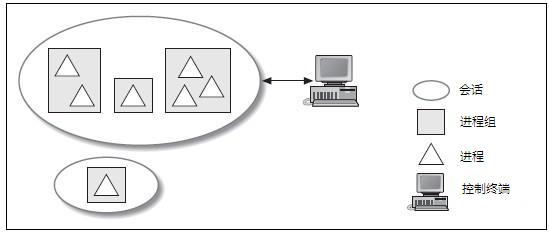
\includegraphics[width=\textwidth]{ch5.jpg}
  \caption{会话、进程组、进程及控制终端之间的关系}
\end{figure}
 
Linux提供了几个用来获取和设置与一个进程相关的会话进程组的接口。它们主要是为shell服务的,但是也可用于像守护进程之类的进程,因为守护进程不希望与与会话和进程组扯上关系。

\subsection{与会话相关的系统调用}

在登陆时,shell会创建新的会话。这是通过一个特殊的系统调用完成的,用它可以很容易的创建一个会话:

\begin{lstlisting}
  #include <unistd.h>
  pid_t setsid (void);
\end{lstlisting}

假如调用进程不是某个进程组组长进程,调用setsid()会创建新的会话。调用进程就是这个会话的唯一进程,也是新会话的首进程,但是它没有控制终端。调用也同时在这个会话中创建一个进程组,调用进程成为了组长进程,也是进程组中的唯一进程。新会话ID和进程组ID被设置为调用进程的pid。

也就是说,setsid()创建的新会话,并在其中创建一个新的进程组,而且使得调用进程成为新会话的首进程和新进程组的组长进程。对于守护进程来说,这十分有用,因为它不想是任何已存在会话的成员,也不想拥有控制终端。对于shell来说,它也很有用,因为shell希望为每一个登陆的用户创建新的会话。

成功调用,setsid()返回新会话的会话ID。错误时,返回-1,并把errno设置为EPERM,表示调用进程是是当前进程组的组长进程。有一个简单的方法可以使得任何进程不成为组长进程。这就是创建一个新进程,终止父进程,让子进程来调用setsid()。例如:

\begin{lstlisting}
  pid_t pid;
  pid = fork ();
  if (pid == -1) {
    perror ("fork");
    return -1;
  } else if (pid != 0)
    exit (EXIT_SUCCESS);
  if (setsid ( ) == -1) {
    perror ("setsid");
    return -1;
  }
\end{lstlisting}

虽然获得当前进程的会话ID不是很常用,但是也是可以做到的:

\begin{lstlisting}
  #define _XOPEN_SOURCE 500
  #include <unistd.h>
  pid_t getsid (pid_t pid);
\end{lstlisting}

对getsid()的调用会返回pid进程的会话ID。如果参数pid是0,就返回调用进程的会话ID。错误时,返回-1。而errno的唯一可能值就是ESRCH,表示pid不代表任何进程。注意,其他UNIX系统会把errno设置为EPREM,它表示pid指示的进程和调用进程不属于同一个会话。Linux不会这么处理,它倾向于返回任何进程的会话ID。

getsid()是很少使用的,且主要用于诊断问题:

\begin{lstlisting}
  pid_t sid;
  sid = getsid (0);
  if (sid == -1)
    perror ("getsid"); /* should not be possible */
  else
    printf ("My session id=%d\n", sid);
\end{lstlisting}

\subsection{与进程组相关的系统调用}

setpgid()将pid进程的进程组ID设置为pgid:

\begin{lstlisting}
  #define _XOPEN_SOURCE 500
  #include <unistd.h>
  int setpgid (pid_t pid, pid_t pgid);
\end{lstlisting}

如果pid是0,则使用调用者的进程ID。如果pgid是0,则将pid的进程ID设置为进程组ID。

成功时,返回0。它必须依赖几个条件:

\begin{itemize}
\item pid代表的进程必须是调用者或者是其子进程,而且子进程没有调用过exec函数,并且pid进程和调用者在同一个会话中。
\item pid进程不能是会话首进程。
\item 如果pgid已经存在,那么必须与调用者在同一个会话中。
\item pgid非负。
\end{itemize}

错误时,返回-1,并把errno设置为下列值之一:

\begin{eqlist*}
\item[\textbf{EACCESS}] pid进程是调用进程的子进程,且调用进程调用了exec函数。
\item[\textbf{EINVAL}] pgid小于0。
\item[\textbf{EPERM}] pid进程是会话首进程,或者是与调用者不在同一个会话中的另一个进程。也可能是试图将进程放置到一个不在同一个会话的进程组中。
\item[\textbf{ESRCH}] pid不是当前进程或0或当前进程的子进程。
\end{eqlist*}

尽管不是很常用,还是可以通过会话获得进程的进程组ID:

\begin{lstlisting}
  #define _XOPEN_SOURCE 500
  #include <unistd.h>
  pid_t getpgid (pid_t pid);
\end{lstlisting}

getpgid()返回pid进程的进程组ID。如果pid是0,返回当前进程的进程组ID。出错则返回-1,而errno的唯一值是ERSCH,表示pid是一个非法的进程标识符。

与getsid()类似,getpgid也主要用于诊断错误:

\begin{lstlisting}
  pid_t pgid;
  pgid = getpgid (0);
  if (pgid == -1)
    perror ("getpgid"); /* should not be possible */
  else
    printf ("My process group id=%d\n", pgid);
\end{lstlisting}

\subsection{废弃的进程组函数}

Linux支持BSD中两个较早的用于操作和获取进程组ID的接口。因为它们不如前面讨论的系统调用常用了,除非对可移植性有要求,新的程序应该不使用它们。setpgrp()用来设置进程组ID:

\begin{lstlisting}
  #include <unistd.h>
  int setpgrp (void);
\end{lstlisting}

这样的调用:

\begin{lstlisting}
  if (setpgrp ( ) == -1)
    perror ("setpgrp");
\end{lstlisting}

和下面的调用是一样的:

\begin{lstlisting}
  if (setpgid (0,0) == -1)
    perror ("setpgid");
\end{lstlisting}

两个都试图把进程组ID设置为当前进程的进程ID。成功时返回0,失败时返回-1。除了ERSCH,setpgid()的所有errno可能值都适用于setpgrp()。

同样的,getpgrp()用来获取进程组ID:

\begin{lstlisting}
  #include <unistd.h>
  pid_t getpgrp (void);
\end{lstlisting}

这样的调用:

\begin{lstlisting}
  pid_t pgid = getpgrp ( );
\end{lstlisting}

和下面的是一样的:
\begin{lstlisting}
  pid_t pgid = getpgid (0);
\end{lstlisting}

两者都返回调用进程的进程组ID。getpgid()不能失败。

\section{守护进程}

守护进程运行在后台,不与任何控制终端相关联。守护进程通常在系统启动时就运行,它们以root用户运行或者其他特殊的用户(例如apache和postfix),并处理一些系统级的任务。习惯上守护进程的名字通常以d结尾(就像crond和sshd),但这不是必须的,甚至不是通用的。

这个名字来源于麦克斯韦妖(Maxwell’s demon),它是物理学家James Maxwell在1867年进行的一个思想实验。Daemon这个词也是希腊神话中的鬼怪,它存在与人类和神之间,拥有占卜的能力。与Judeo-Christian神话中的daemon不同,希腊神话中的daemon不是邪恶的。实际上,神话中的daemon是神的助手,做一些奥林匹斯山的居民自己不愿做的事——很像Unix中的守护进程,完成前台用户不愿做的事。

对于守护进程有两个基本要求:它必须是init进程的子进程,并且不与任何控制终端相关联。

一般来讲,进程可以通过以下步骤成为守护进程:

\begin{enumerate}
\item 调用fork(),创建新的进程,它会是将来的守护进程。
\item 在守护进程的父进程中调用exit()。这保证了祖父进程(守护进程的祖父进程)确认父进程已经结束。还保证了父进程不再继续运行,守护进程不是组长进程。最后一点是顺利完成以下步骤的前提。
\item 调用setsid(),使得守护进程有一个新的进程组和新的会话,两者都把它作为首进程。这也保证它不会与控制终端相关联(因为进程刚刚创建了新的会话,同时也就不会为其关联一个控制终端)。
\item 用chdir( )将当前工作目录改为根目录。因为前面调用fork()创建了新进程,它所继承来的当前工作目录可能在文件系统中任何地方。而守护进程通常在系统启动时运行,同时不希望一些随机目录保持打开状态,也就阻止了管理员卸载守护进程工作目录所在的那个文件系统。
\item 关闭所有的文件描述符。不需要继承任何打开的文件描述符,对于无法确认的文件描述符,让它们继续处于打开状态。
\item 打开0、1和2号文件描述符(标准输入、标准输出和标准错误),把它们重定向到/dev/null。
\end{enumerate}

根据这些规则,下面的程序可以成为守护进程:

\begin{lstlisting}
  #include <sys/types.h>
  #include <sys/stat.h>
  #include <stdlib.h>
  #include <stdio.h>
  #include <fcntl.h>
  #include <unistd.h>
  #include <linux/fs.h>
  int main (void)
  {
    pid_t pid;
    int i;
    /* create new process */
    pid = fork ( );
    if (pid == -1)
      return -1;
    else if (pid != 0)
      exit (EXIT_SUCCESS);
    /* create new session and process group */
    if (setsid ( ) == -1)
      return -1;
    /* set the working directory to the root directory */
    if (chdir ("/") == -1)
      return -1;
    /* close all open files--NR_OPEN is overkill, but works */
    for (i = 0; i < NR_OPEN; i++)
      close (i);
    /* redirect fd's 0,1,2 to /dev/null */
    open ("/dev/null", O_RDWR);     /* stdin */
    dup (0);                        /* stdout */
    dup (0);                        /* stderror */
    /* do its daemon thing... */
    return 0;
  }
\end{lstlisting}

许多Unix系统在它们的C函数库中提供了daemon()函数来完成这些工作,将繁琐的工作简化了很多:

\begin{lstlisting}
  #include <unistd.h>
  int daemon (int nochdir, int noclose);
\end{lstlisting}

如果nochdir非零,就不会将工作目录改为根目录。如果noclose非零,就不关闭所有打开的文件描述符。如果父进程设置了守护进程的这些属性,那么这些参数是很有用的。通常都会把这些参数设为0。

成功时,返回0。失败时返回-1。errno设置为fork()或者setsid()的错误代码之一。

\section{总结}

在本章中,我们讲解了Unix系统中进程管理的基本知识,包括了从进程的创建到进程的终止。下一章,我们会讲解一些高级进程管理的API,例如改变进程调度方式的的API。
